\documentclass[10pt]{beamer}
\usetheme[
%%% option passed to the outer theme
%    progressstyle=fixedCircCnt,   % fixedCircCnt, movingCircCnt (moving is deault)
  ]{Feather}
  
% If you want to change the colors of the various elements in the theme, edit and uncomment the following lines
\definecolor{grey}{rgb}{0.52, 0.52, 0.51}

% Change the bar colors:
\setbeamercolor{Feather}{fg=grey!20,bg=grey}
% This is the inner theme file of the Feather theme.
% Copyright (c) 2014 by Lilyana Vaskova Vankova <lilqna.v@gmail.com>
%
% This program is free software: you can redistribute it and/or modify
% it under the terms of the GNU General Public License as published by
% the Free Software Foundation, either version 3 of the License, or
% (at your option) any later version.
%
% This program is distributed in the hope that it will be useful,
% but WITHOUT ANY WARRANTY; without even the implied warranty of
% MERCHANTABILITY or FITNESS FOR A PARTICULAR PURPOSE.  See the
% GNU General Public License for more details.
%
% You can find the GNU General Public License at <http://www.gnu.org/licenses/>.

%----------------------------------------------------------------------------------------------------------------------------------

\NeedsTeXFormat{LaTeX2e}
\ProvidesPackage{beamerinnerthemeFeather}[2014/04/08 v1.0.0 The Feather Beamer Theme]

%----------------------------------------------------------------------------------------------------------------------------------

%%%%%%%%%%%%%%%%%%%%%%%%%%%%%%%%%%%%%%%%%%%%%%%%
% Theme options, definitions and templates.
%%%%%%%%%%%%%%%%%%%%%%%%%%%%%%%%%%%%%%%%%%%%%%%%

%----------------------------------------------------------------------------------------------------------------------------------

% beamer specific options

               \mode<presentation> %refers to the first four modes (beamer,handout,second and trans). That is, to all modes except the article mode
{

%----------------------------------------------------------------------------------------------------------------------------------

% title page
%% definitions for fonts of the different elements
  
               \setbeamerfont{institute}{family=\rmfamily, size = \footnotesize}
               \setbeamerfont{title}{family=\rmfamily, size = \huge} 
               \setbeamerfont{subtitle}{family=\rmfamily, size = \Large}
               \setbeamerfont{author}{family=\rmfamily, size = \footnotesize}
               \setbeamerfont{date}{family=\rmfamily, size = \footnotesize}

               \setbeamertemplate{title page}
   {

%% setting the above definitions

        \begin{minipage}[c][\textheight][c]{\textwidth}

                  \centering

                 {\usebeamerfont{institute}\insertinstitute}\vspace*{30pt}

                 {\usebeamerfont{title}\usebeamercolor[fg]{title}\inserttitle}\vspace*{10pt}

                 {\usebeamerfont{subtitle}\usebeamercolor[fg]{subtitle}\insertsubtitle}\vspace*{30pt}

                 {\usebeamerfont{author}\insertauthor}\vspace*{30pt}

                 {\usebeamerfont{date}\insertdate}\vspace*{\baselineskip}

         \end{minipage}
   }
  
%----------------------------------------------------------------------------------------------------------------------------------
  
% final page

                  \defbeamertemplate{final page}{text}[1]
   {
         \begin{minipage}[c][\textheight][c]{\textwidth}
                  \centering
                  #1
         \end{minipage}
   }
                  \newcommand{\finalpage}[1]
   {
                  \setbeamertemplate{final page}[text]{#1}
                  \usebeamertemplate{final page}
   }

%----------------------------------------------------------------------------------------------------------------------------------
  
% add the feather to the background of the titlepage and the final page

                  \newcommand{\1}
   {
                  \setbeamertemplate{background}
      {
                  
\includegraphics[height=\paperheight]{Feathergraphics/1}
                  \tikz[overlay] \fill[fill opacity=0.8,fill=white] (0,0) rectangle (-\paperwidth,\paperheight);
       }
    }

%----------------------------------------------------------------------------------------------------------------------------------
  
% use numbers instead of a picture for the references

                  \setbeamertemplate{bibliography item}[text]

}

\mode<all>
% Change the color of the structural elements:
\setbeamercolor{structure}{fg=grey}

% Change the frame title text color:
%\setbeamercolor{frametitle}{fg=blue}

% Change the normal text color background:
\setbeamercolor{normal text}{fg=black,bg=gray!10}

%-------------------------------------------------------
% INCLUDE PACKAGES
%-------------------------------------------------------

\usepackage[utf8]{inputenc}
\usepackage[english]{babel}
\usepackage[T1]{fontenc}
\usepackage{helvet}


%-------------------------------------------------------
% DEFFINING AND REDEFINING COMMANDS
%-------------------------------------------------------

% colored hyperlinks
\newcommand{\chref}[2]{
  \href{#1}{{\usebeamercolor[bg]{Feather}#2}}
}

%-------------------------------------------------------
% INFORMATION IN THE TITLE PAGE
%-------------------------------------------------------

\title[] % [] is optional - is placed on the bottom of the sidebar on every slide
{ % is placed on the title page
      \textbf{Wavelength}
}

\subtitle[$\lambda$-IDE]
{
      \textbf{$\lambda$-IDE}
}

\author[wavelength]
{      Muhammet Guemues \\
	   \textbf{Jean-Pierre von der Heydt} \\
       \textbf{Markus Himmel} \\
       Marc Huisinga \\
       Philip Klemens \\ 
       \textbf{Julia Schmid} \\       
}

\institute[]
{
      
  
  %there must be an empty line above this line - otherwise some unwanted space is added between the university and the country (I do not know why;( )
}

\date{\today}

%-------------------------------------------------------
% THE BODY OF THE PRESENTATION
%-------------------------------------------------------

\begin{document}

%-------------------------------------------------------
% THE TITLEPAGE
%-------------------------------------------------------

{\1% % this is the name of the PDF file for the background
\begin{frame}[plain,noframenumbering] % the plain option removes the header from the title page, noframenumbering removes the numbering of this frame only
  \titlepage % call the title page information from above
\end{frame}}

\begin{frame}{$\lambda$-IDE}{}
	\begin{overprint}
    \onslide<1>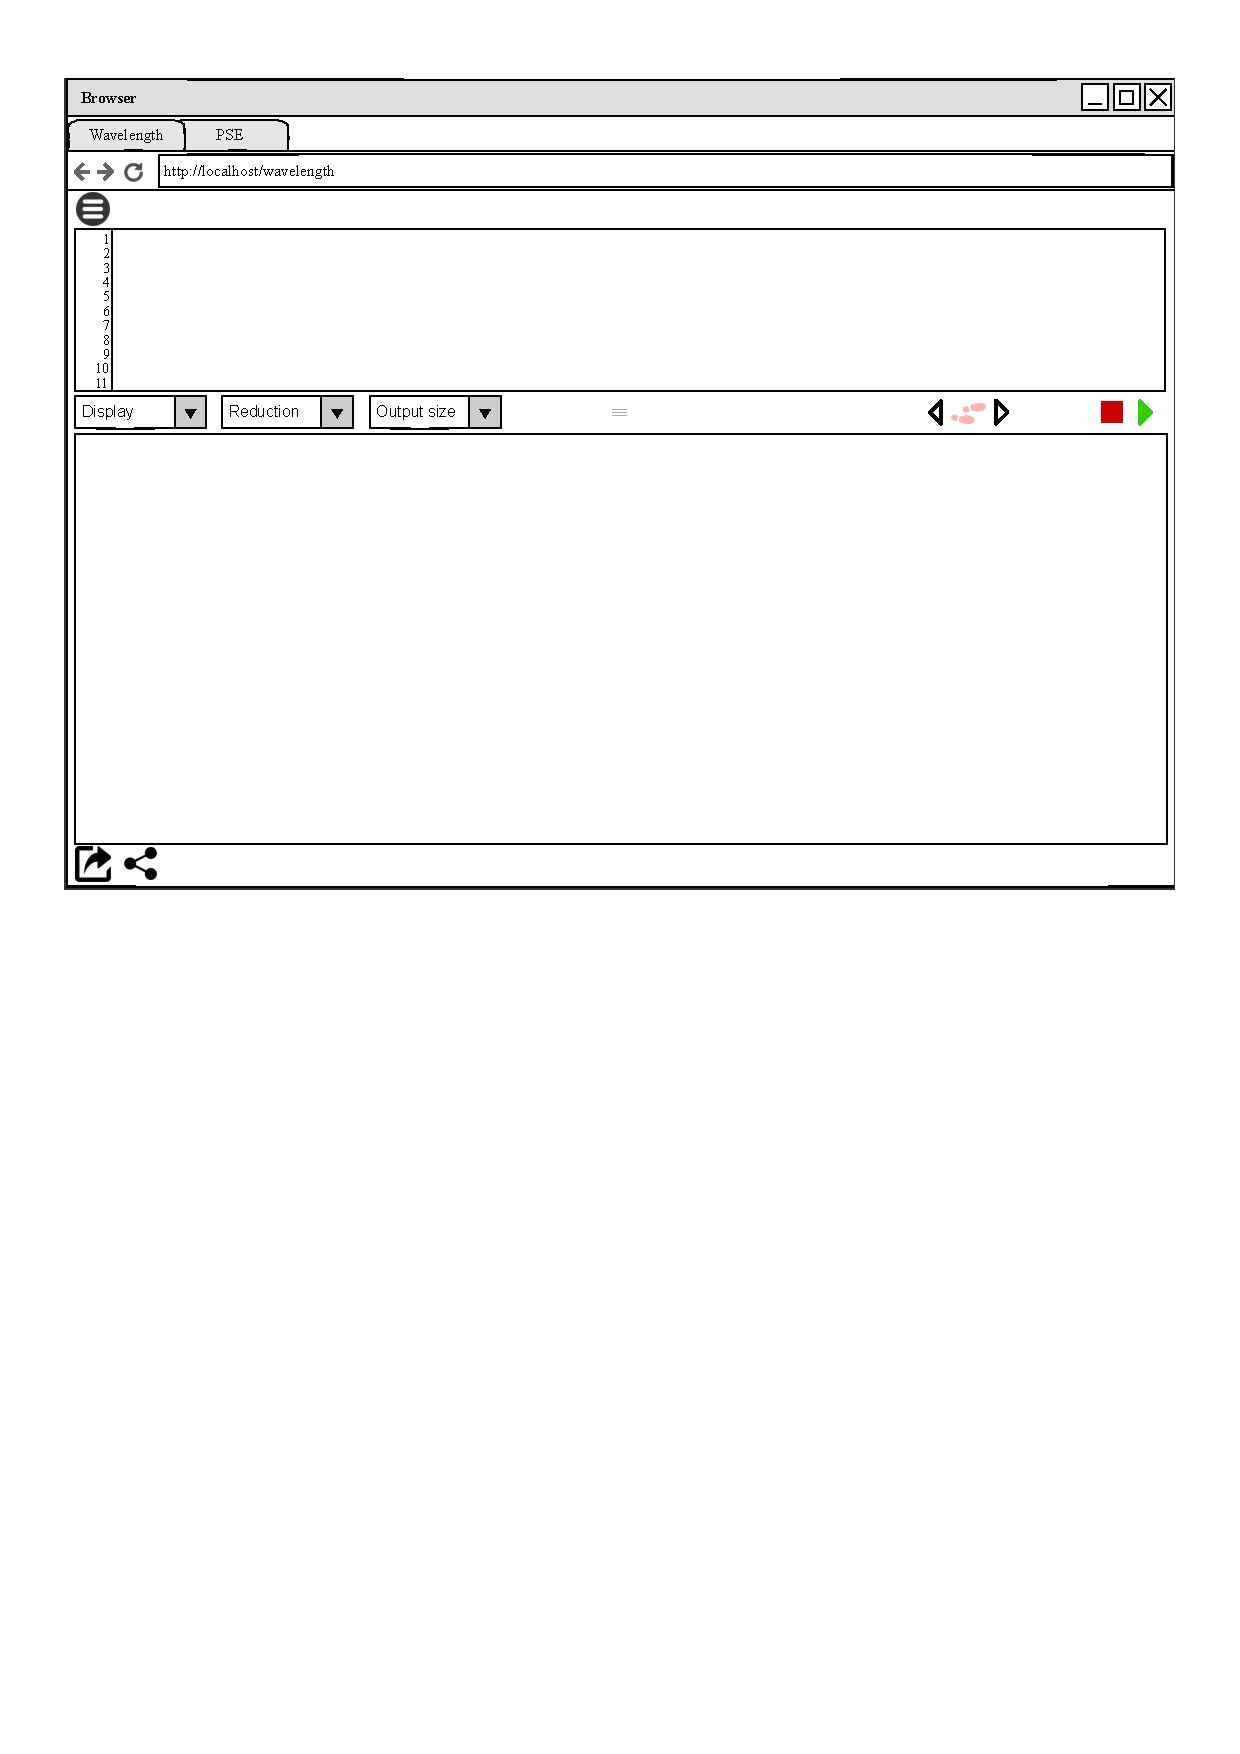
\includegraphics[scale = 0.5]{img/startseite}
    \onslide<2>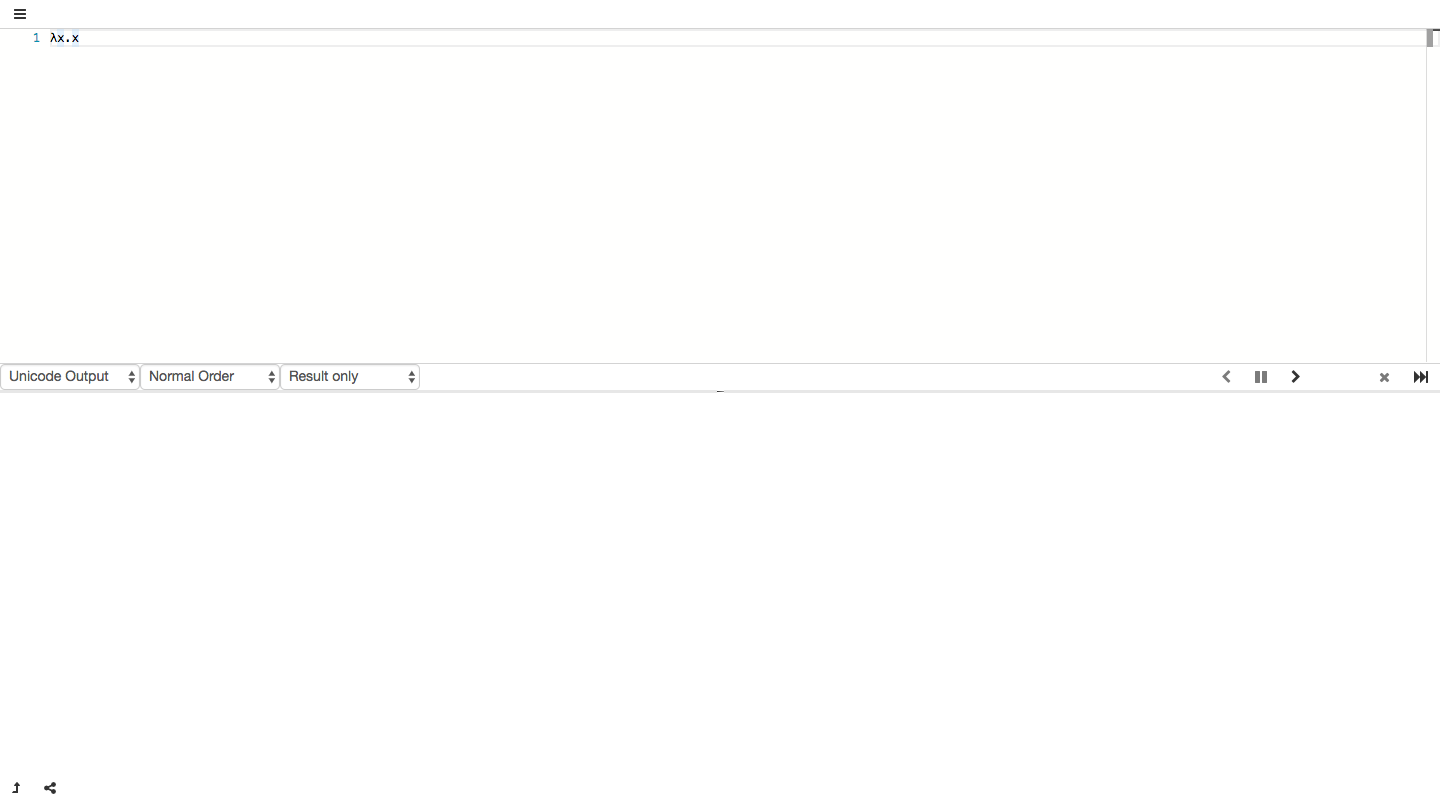
\includegraphics[scale = 0.2]{img/GUI}
    \end{overprint}
\end{frame}


\begin{frame}{Statistiken}{}
	\begin{itemize}
		\item Lines of Code: 10.208
		\begin{itemize}
			\item Java: 9.644
			\item JavaScript: 269
			\item CSS: 295
		\end{itemize}
		\item Anzahl Klassen: 116
		\item Anzahl Packages: 19
		\item Lines of Testcode: 5809 
		\item Anzahl Git-Commits: 1.032, Tendenz steigend
	\end{itemize}
	
	\begin{overprint}
    \onslide<1>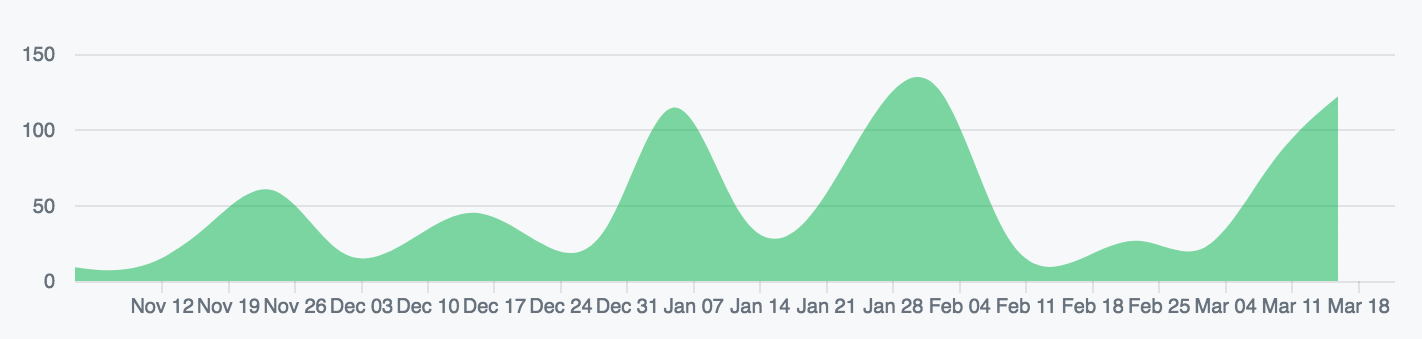
\includegraphics[width = \textwidth]{img/GitCommits}
    \onslide<2>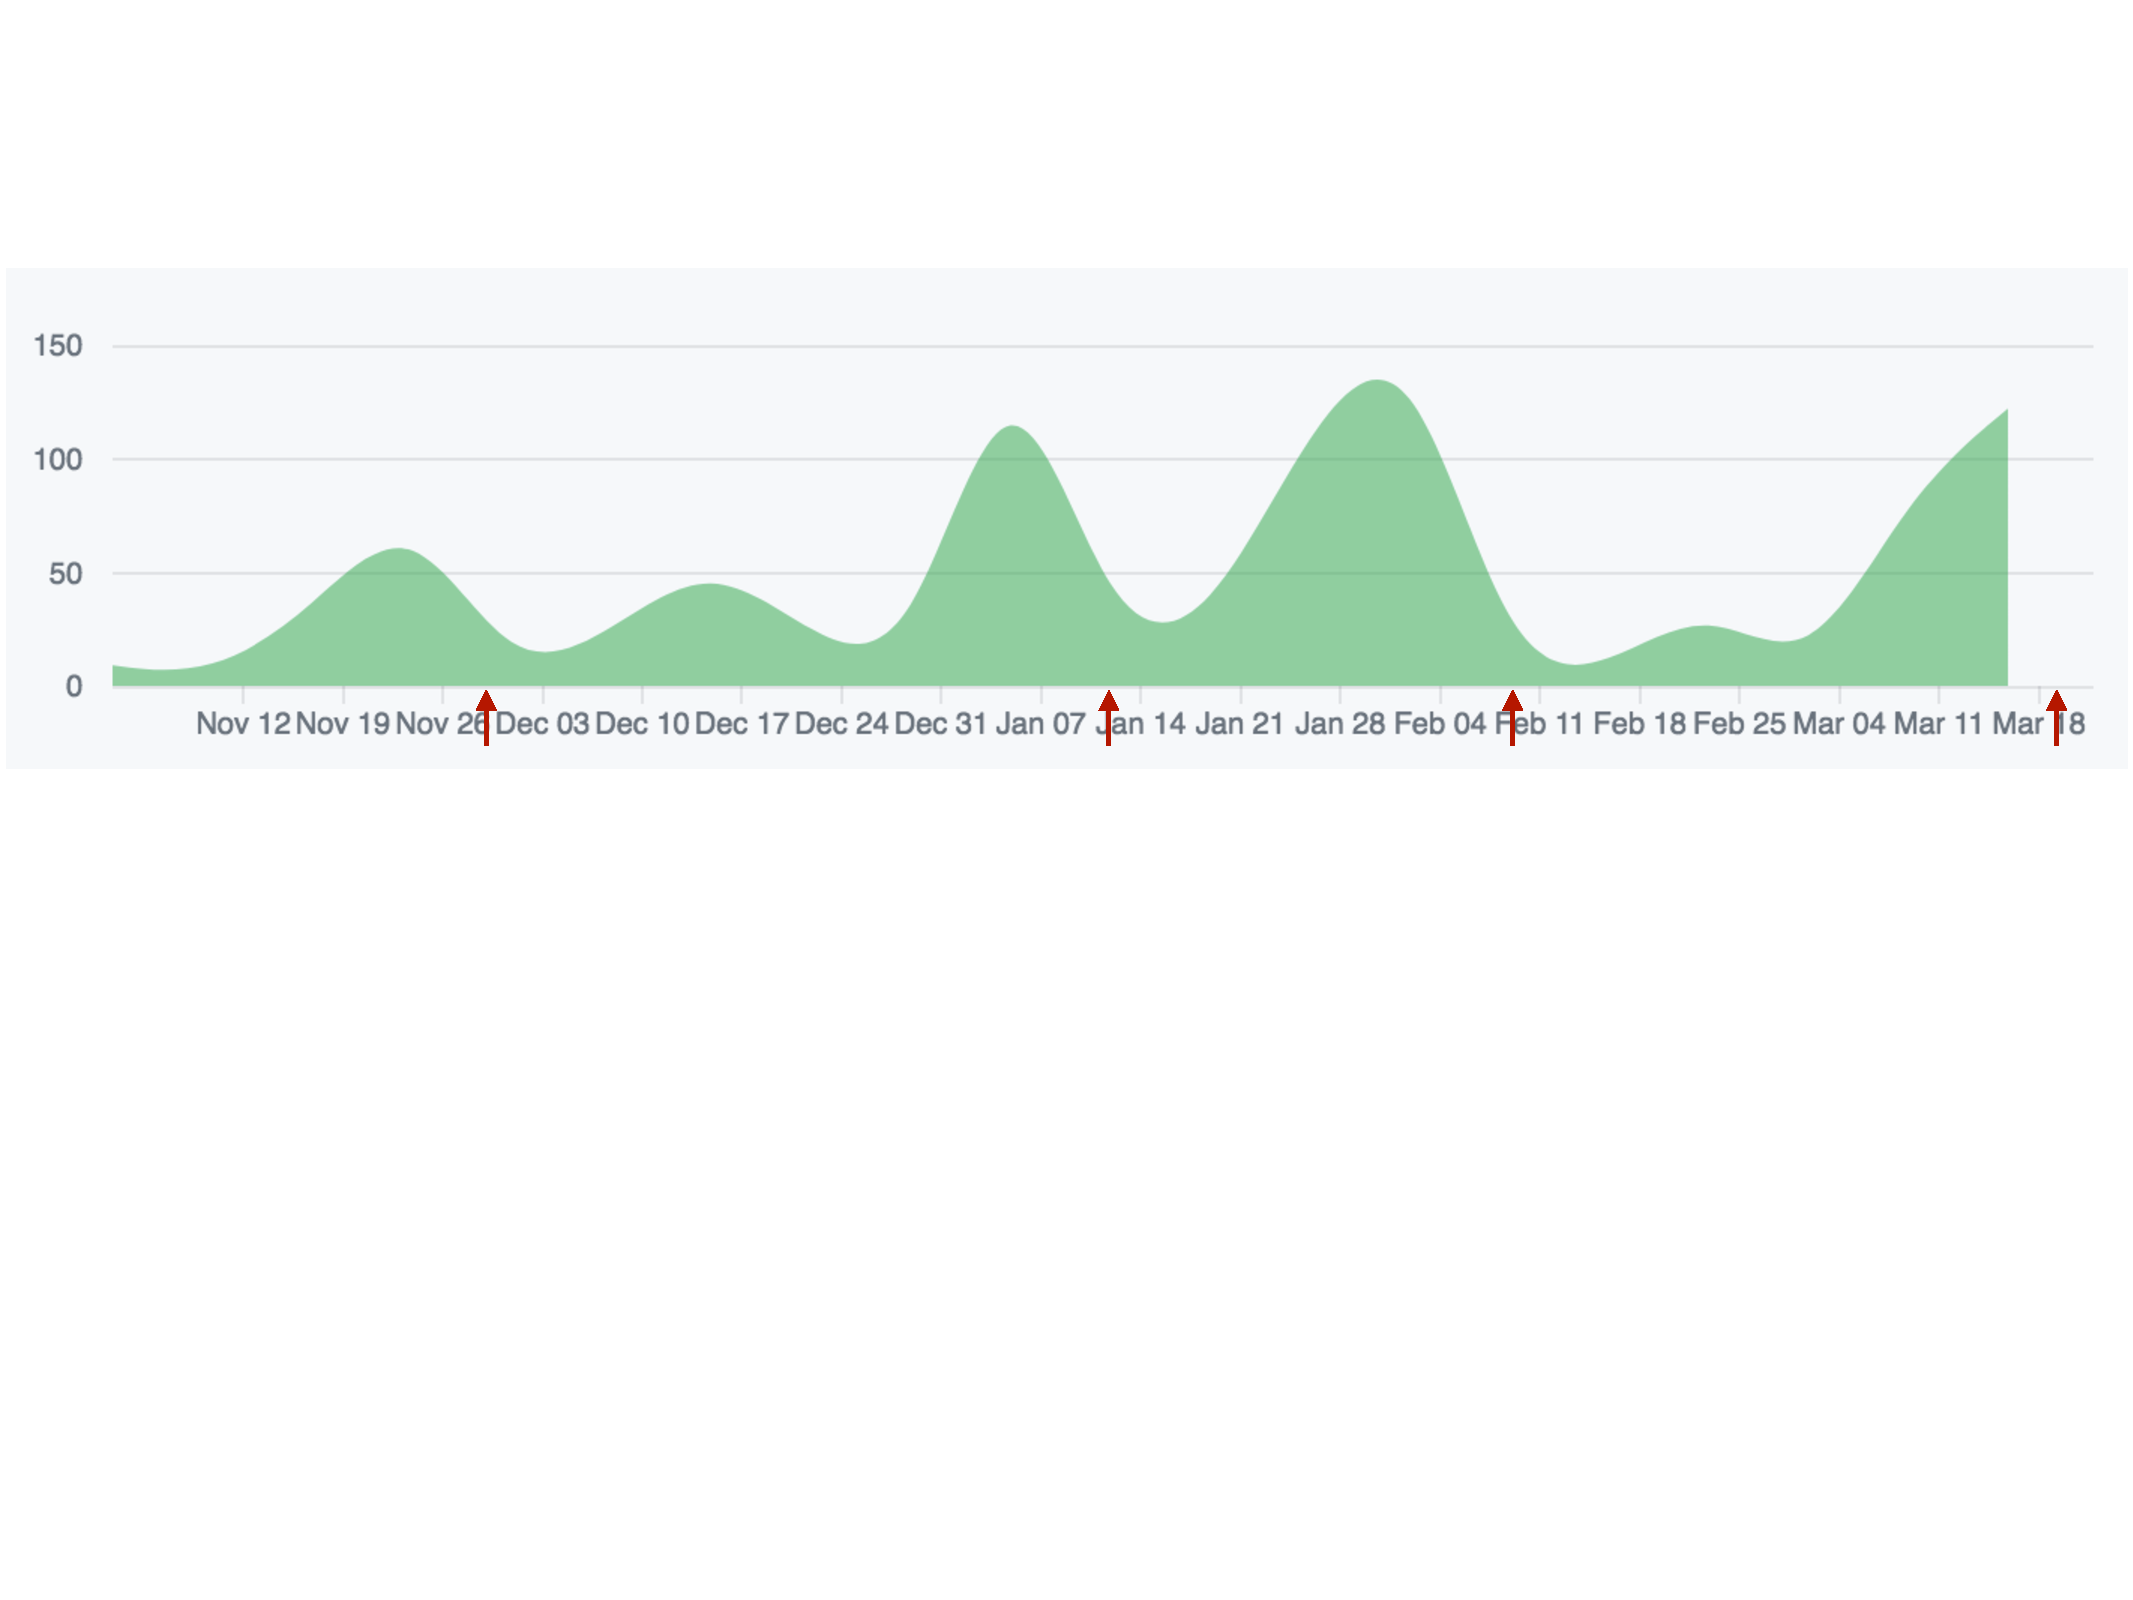
\includegraphics[width = \textwidth]{img/GitCommitsWithApp}
    \end{overprint}
\end{frame}


\begin{frame}{Tools und Bibliotheken}{}
	\begin{itemize}
		\item Pencil
		\item PlantUML
		\item Doclet
		\item GWT
		\item Eclipse
		\item GWT Eclipse Plugin
		\item GWT Bootstrap
		\item SQLite
		\item JUnit
		\item vis.js
		\item Monaco
		\item Selenium
	\end{itemize}
\end{frame}

\begin{frame}{Tools}{Pencil}
	\begin{itemize}
		\item UI Design Tool
		\item Probleme:
			\begin{itemize}
				\item Layering nicht möglich
				\item lustige Bugs bei pdf Export
			\end{itemize} 
	\end{itemize}
\end{frame}

\begin{frame}{Tools}{PlantUML}
	\begin{itemize}
		\item UML Sequenzdiagramme
		\item UML Klassen-Diagramme aus Java Code
		\item Problem: 
			\begin{itemize}
				\item schlechtes Layout bei Klassendiagrammen $\rightarrow$ Inkscape
			\end{itemize}
	\end{itemize}
\end{frame}

\begin{frame}{Tools}{Doclet}
	\begin{itemize}
		\item sammelt Java-Doc aus Java Projekt in \LaTeX \ Datei
		\item eigenes Doclet geschrieben
	\end{itemize}
\end{frame

\begin{frame}{Tools}{GWT}
	\begin{itemize}
		\item GWT: Java zu JavaScript Transpiler 
		\item Probleme: 
		\begin{itemize}
			\item Komponenten $\rightarrow$ GWTBootstrap
			\item Java Standardfunktionen nicht verfügbar
		\end{itemize}
	\end{itemize}
\end{frame}

\begin{frame}{Tools}{Eclipse und GWT Plugin}
	\begin{itemize}
		\item Änderungen im Development-Mode  
		\item Probleme:
		\begin{itemize}
			\item hochgradig nichtdeterministisches Verhalten
		\end{itemize}
	\end{itemize}
\end{frame}


\begin{frame}{Bibliotheken}{vis.js}
	\begin{itemize}
		\item Grafikbibliothek zur Datenvisualisierung
		\item Probleme: 
			\begin{itemize}
				\item{Baumbreite}
				\item{Terme anklicken}
			\end{itemize}
	\end{itemize}
\end{frame}

\begin{frame}{Review}{}
	\begin{itemize}
		\item UI-Planung zu Beginn
		\item UI-Prototyp
		\item Implementieren in Entwurfsphase
		\item Merge-Tag
	\end{itemize}
	
\end{frame}

{\1
\begin{frame}[plain,noframenumbering]
  \finalpage{DANKE}
\end{frame}}

\end{document}